\documentclass[11pt,english]{article}
%\usepackage[a4paper,margin=24mm]{geometry}
\usepackage[a4paper]{geometry}

\title{DT167G Software Security VT17\\Group Project}
\author{Alexander Gillberg (algi1701), Gustaf Holst (guho1700), Michaela Hörnfeldt (mihr1401)\\Anders Jensen-Urstad (anje0901), Zahra Zaree (zaza1400)}
\date{2019-06-02}

\usepackage{booktabs}

\usepackage{polyglossia}
\setdefaultlanguage{english}
\usepackage{csquotes}
\MakeOuterQuote{"}
\usepackage{icomma}

\usepackage[usenames,dvipsnames,svgnames]{xcolor}

\usepackage{graphicx}
\graphicspath{{graphics/}}
\usepackage{eso-pic}
\usepackage{wrapfig}

\usepackage{minted}

\usepackage{hyperref}
\makeatletter
\hypersetup{pdftex, colorlinks=true, linkcolor=DarkRed, filecolor=blue, urlcolor=DarkRed, pdftitle={\@title}, pdfauthor={\@author}, pdfsubject=, pdfkeywords=}
\makeatother

\usepackage{fontspec}
\setmainfont{Minion Pro}
\setmonofont[Scale=0.8]{DejaVu Sans Mono}
\usepackage{textcomp}

\usepackage{listings}
\lstset{basicstyle=\ttfamily\footnotesize,breaklines=true}

\usepackage{setspace}
%\onehalfspacing
\usepackage{xunicode}

\usepackage{titling}
\renewcommand\maketitlehooka{\null\mbox{}\vfill}
\renewcommand\maketitlehookd{\vfill\null}

\usepackage{etoolbox}
\makeatletter
\patchcmd{\@maketitle}{\begin{center}}{\begin{flushleft}}{}{}
\patchcmd{\@maketitle}{\begin{tabular}[t]{c}}{\begin{tabular}[t]{@{}l}}{}{}
\patchcmd{\@maketitle}{\end{center}}{\end{flushleft}}{}{}
\makeatother

\AddToShipoutPictureBG*{%
  \AtTextUpperLeft{% Position at upper left of text block
    \hspace*{\textwidth}% Move over to upper right of text block
    \llap{% Ignore horizontal width and overlap to the left
      \smash{% Ignore vertical height
        \raisebox{-1.1\height}{% Lower so top touches baseline
            
\includegraphics[width=5cm,keepaspectratio]{miun}}}}}}

\newcommand\ftnote[1]{\footnote{\raggedright#1}}

\begin{document}

\begin{titlingpage}
\maketitle
\end{titlingpage}

\section{Background}
Considering the fact that the foundation for our modern day Internet was established in a time when only a few thousand computers were connected to it and security matters were way down on the list of concerns, it is astonishing that it still, more or less, works at all. Through the years partial solutions and temporary fixes have been padded on to the system attempting to accommodate the big explosion in number of connected devices as well as new technologies added to the mix.

The world wide web has become a snake pit of security issues, and creating a secure web application is not a trivial task. Once an application is made available online it will be open for attacks from malicious and/or ignorant users. The consequences of a successful attack are not necessarily limited to the owner of the application but can have ramifications for its unsuspecting users as well. That is why publishing an application on the Internet should be considered a great responsibility which needs to be taken seriously.

The skills of potential attackers range from very basic to very, very advanced. Some attacks require very little knowledge to carry out, but are also relatively easy to protect against and it becomes mostly a matter of remembering to take the necessary precautions. To facilitate building safe(r) web applications the developer community is constantly creating new, and refining old, tools in the form of frameworks and libraries that are intended to take care of those common pitfalls, effectively giving the developer more time to focus on the actual functionality of the application.

\section{Purpose}

The purpose is to build a Twitter-like web application with any language/framework. The requirements are as follows:

\begin{itemize}
  \item Users should be able to register
  \item Users should be able to post messages if logged in
  \item Users should able to upvote/downvote messages if logged in
  \item It must be possible to search/filter messages by user, word in message, or a combination thereof
  \item Users should be able to delete their own messages
\end{itemize}

\section{Design and implementation}
Early on it was agreed upon within the group that the most effective and secure way to build a site like this is using an existing framework. One of the mantras of web development security goes “don’t roll your own”. During the years many people have already put a lot of work into developing and testing solutions to the common security issues with a modern web app, solutions that have then also proven themselves by standing the test of time. Those solution are most certainly better and more secure than anything we would be able to create in two weeks.

Thus, work began by choosing a language/framework combination for the project. Two such combinations were considered, namely PHP/Laravel\footnote{\url{https://laravel.com/}} and Python/Django\footnote{\url{https://www.djangoproject.com/}}. The final choice fell on Python and Django, since some of the group members had previous experience with Django, and there was a general preference for Python over PHP.

Django is a high-level, free and open source web framework written in Python made for database-driven websites. It follows a “batteries included” approach, meaning virtually all the most common components such sites typically need are included out of the box: object-relational mapper, form serialization/validation, template system, authentication framework, mitigation against various common attacks turned on by default, etc.

\subsection{Frontend}

The main focus on the project was the security aspects of the assignment. To minimize the time spent on the frontend (more time solving security issues/backend stuff) the open source CSS framework Bootstrap\footnote{\url{https://getbootstrap.com/}} was used. It provided easy and fast development. With templates for typography, forms, buttons and other user interface components that Bootstrap provides, as well as different ready-to-use themes, the frontend was done in a second with minimal effort.

\subsection{Backend}

For user authentication we use Django’s own system,\footnote{\url{https://docs.djangoproject.com/en/2.2/ref/contrib/auth/}} which also provides a default User model. To represent tweets (posts) and votes two models, Post and Vote, were added.

Since Django has been around for a long time and is very popular, many ready-made “apps” that can easily be plugged into any Django project are available. We make use of several:

\begin{itemize}
  \item django-registration\footnote{\url{https://pypi.org/project/django-registration/}} to enable creation of new accounts
  \item django-two-factor-auth\footnote{\url{https://pypi.org/project/django-two-factor-auth/}} to provide optional two-factor authentication
  \item django-useraudit\footnote{\url{https://pypi.org/project/django-useraudit/}} to log login attempts (whether successful or not)
  \item django-ratelimit\footnote{\url{https://pypi.org/project/django-ratelimit/}} to rate-limit various things
  \item argon2-cffi\footnote{\url{https://pypi.org/project/argon2-cffi/}} to use the Argon2 password hasher
\end{itemize}

Most of the time was then spent writing views (a view simply being a function or class that takes a request and returns a response) -- for example, one view to handle post creation, one to handle searching, etc. -- and hooking them up to templates and mapping URLs to views.

SQLite is used as the database backend, as it requires no external dependencies. Changing it for another DBMS is a simple matter thanks to Django's ORM. For a production website it is probably wise to use a dbms that, for example, supports concurrent writes.

\section{Evaluation of security}

\subsection{Cross-site scripting (XSS)}

To avoid cross-site scripting (XSS), all user-provided data (e.g. tweets) shown on HTML pages goes through Django’s template system, which automatically escapes all <, >, ‘, “ and \& characters (they are converted to their respective HTML entities).\footnote{\url{https://docs.djangoproject.com/en/2.2/ref/templates/language/\#automatic-html-escaping}} For example, if a user posts the following:

\begin{minted}[fontsize=\footnotesize]{html}
<script>alert('wee');</script>}
\end{minted}

It will be stored as-is in the database but output as:

\begin{minted}[fontsize=\footnotesize]{html}
&lt;script&gt;alert(&#39;wee&#39;);&lt;/script&gt;
\end{minted}

Additionally, as an added layer of security, we use a strict CSP (Content-Security-Policy) policy (\lstinline{default-src 'self'}). Among other things, this blocks inline JavaScript and CSS, so even if someone did manage to get unescaped code onto the site, any modern browser would refuse to execute it. This is done in the HeadersForGreatJustice middleware (\lstinline{tweets/middleware.py}). For example, if \lstinline{<script>alert('wee');</script>} appeared in the page somewhere, Firefox refuses to run it with the following message:

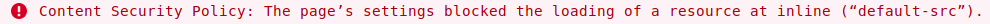
\includegraphics[width=\textwidth]{csp_violation}

\subsection{Cross-site request forgery (CSRF)}

To avoid cross-site request forgery (CSRF), Django’s built-in protection is used. When a user logs in, a CSRF cookie (a secret plus a random salt) is set . Every form that does a POST request has a hidden field with another CSRF token: same secret, but with a salt that’s regenerated every time the form is loaded, so it’s never the same across page loads. When the form is submitted, the server checks that the secret in the cookie matches the secret in the form field.\footnote{\url{https://docs.djangoproject.com/en/2.2/ref/csrf/}}

\subsection{SQL injections}

Django's own object-relational mapper (ORM) is used as a database abstraction layer. It makes use of parameterized queries (a.k.a. prepared statements), which means an SQL query (code) is sent separately from the values (data) used in it. In other words, code and data is not mixed. This prevents SQL injections. We do all database interaction through the ORM and don’t use any raw queries.\footnote{\url{https://docs.djangoproject.com/en/2.2/topics/security/\#sql-injection-protection}}

\subsection{Clickjacking}

Clickjacking is when users are tricked into "clicking a button, a link or a picture, etc. that the web user didn’t intend to click, typically by overlaying the web page with an iframe"\footnote{\url{https://blog.qualys.com/securitylabs/2012/11/29/clickjacking-an-overlooked-web-security-hole}}. We protect against this by sending the X-Frame-Options header with the value DENY, which tells the user’s browser never to allow embedding Tweetstorm in an iframe/frame/embed/object element. This is done with Django’s \lstinline{django.middleware.clickjacking.XFrameOptionsMiddleware}.

\subsection{Brute-force attacks}

\subsubsection{Password validators}

It is common practice for websites to try to aid their users in choosing strong passwords. Many times these attempts end up making the passwords more predictable, because the enforced policy is too specific. Therefore the specifications for Tweetstorm passwords are kept relatively loose. We use Django’s default validators:

\begin{itemize}
  \item\emph{Your password can't be too similar to your other personal information.} The password is checked against username and email.\footnote{\url{https://docs.djangoproject.com/en/2.2/topics/auth/passwords/\#django.contrib.auth.password__validation.UserAttributeSimilarityValidator}} For example, if the username is foobar, the password “foobar2000” is not allowed.
  \item\emph{Your password must contain at least 9 characters.} Passwords must be at least 9 characters and no more than 4096 characters (or, more specifically, no more than 4096 bytes). The upper limit was introduced by Django to prevent a possible Denial of Service attack.\footnote{\url{https://www.djangoproject.com/weblog/2013/sep/15/security/}}
  \item\emph{Your password can't be a commonly used password.} Django checks the password against a list of 20000 common passwords, based on “Top 20K hashes from the Troy Hunt / haveibeenpwned Pwned Passwords list v2 (2018-02-21)”.\footnote{\url{https://gist.github.com/roycewilliams/281ce539915a947a23db17137d91aeb7}}\footnote{\url{https://docs.djangoproject.com/en/2.2/topics/auth/passwords/\#django.contrib.auth.password\_validation.CommonPasswordValidator}}
  \item\emph{Your password can't be entirely numeric.} Self-explanatory.\footnote{\url{https://docs.djangoproject.com/en/2.2/topics/auth/passwords/\#django.contrib.auth.password\_validation.NumericPasswordValidator}}
\end{itemize}

\subsubsection{Rate-limiting}
In order to prevent so called brute force attacks the number of login attempts is limited to 5 per hour for a given username and IP address combination. (If we limited only based on username, a malicious person could intentionally lock out a user. If we limited only based on IP, a malicious person could intentionally lock out others who might share the same public IP address.)

For this we use django-ratelimit\footnote{\url{https://pypi.org/project/django-ratelimit/}}. From \lstinline{tweets/views.py}:

\begin{minted}[fontsize=\footnotesize]{python}
class CustomLoginView(RatelimitMixin, TwoFactorLoginView):
    """Subclass of login view to add rate limiting."""
    ratelimit_key = username_and_ip
    ratelimit_rate = '5/h'
    ratelimit_block = True
    ratelimit_method = 'POST'
\end{minted}

\subsubsection{Hashing}

The password hashing function used is Argon2, winner of the 2015 Password Hashing Competition,\footnote{\url{https://password-hashing.net/}} designed to be computationally expensive. This is defined in \lstinline{tweetstorm/settings.py}.\footnote{\url{https://docs.djangoproject.com/en/2.2/topics/auth/passwords/\#using-argon2-with-django}}

\subsection{Stolen credentials}

Users can optionally enable two-factor authentication, which provides some protection against the situation where someone else has come into possession of their password through, for example, phishing, man-in-the-middle attacks, “shoulder surfing”, etc. With this enabled, the password (what they “know”) alone is not enough to log in: the second factor (what they “have”) must also be provided.

In our case, to make things simple since this is basically just a “proof of concept”, the only second factor supported is one-time passwords (OTP, specifically TOTP, Time-Based One-Time Password\footnote{\url{https://tools.ietf.org/html/rfc6238}}). This is done through the use of django-two-factor-auth which itself is built on top of django-otp.\footnote{\url{https://pypi.org/project/django-otp/}}

To use this a user would typically install an app such as Google Authenticator or FreeOTP on their phone. After logging in on Tweetstorm they can then go to \emph{Account security} -> \emph{Enable two-factor authentication}. Here they are given a QR code -- a key -- which must be scanned using the phone’s OTP app, and which is then saved to the phone. The phone and the Tweetstorm server then both know this secret key.

When logging in next time, after providing the normal password, the user is asked for a token generated by the OTP app on their phone. This token is generated using a combination of the key and the current time. This combination is run through a secure hash function, and from this a six-digit code is derived. This is what the user has to enter. A code is valid for only 30 seconds, and only the phone and and server know what the correct code at any given moment should be.

On the login page an option is given to reset forgotten passwords. This is done by the user providing an email address to which then a link containing a token is sent. Following this link presents the user with a form for resetting the password. If the email address does not exist in the system no error message is displayed, the user is merely informed that an email has been sent (even if it hasn’t). This way an attacker can not draw any conclusions about whether email addresses exist in the database or not by making password reset requests.

\section{Things we don't do}

Use of HTTPS (and secure cookies, Strict Transport Security, etc.) should of course be \emph{absolutely mandatory} on a site like this, but for local development environments a self-signed certificate would cause trust issues unless some extra fiddling is done. So to make it easier for others to test we don’t use HTTPS in VirtualBox image provided.

Many other things could be implemented, but were not, because there’s only so much you can do in two weeks. For example, for people who don’t bother setting up 2FA, we could try to detect previously unseen devices and/or locations and, when triggered, send a code by email that the user would have to enter. We could let a user enter a public PGP key and then encrypt all emails to that user (e.g. password reset, ..) with the user’s key. We could have the login cookie only last for the duration of the browser session by default, and have a “Remember me” checkbox in the sign-in form. We could easily have a two-step workflow for registration, where users would have to click on a confirmation link sent by email to activate their account, but decided not to do that for the sake of easier testing.

Thorough testing is an important part of securing a web app. If more time had been available the project could have been implemented using test-driven development in order to (try to) make sure that no security holes were left unplugged. An extensive test suite would give the team a lot of confidence that the app is doing what it is supposed to to do, even after some changes, major or minor, are made.

\section{Summary and conclusion}

Constructing this site one has been made painfully aware of the difficulties in creating a secure web app. Although the risks might have been theoretically understood it is probably not until you are actually faced with the task you realize the amount of care that needs to be taken with every detail. Obviously Django is taking care of many of the actual implementation details but the developer still has to be aware and make sure the right tools are used and the right measurements are taken for the specific application.

\end{document}